\documentclass[a4paper,12pt]{report}
\usepackage{graphicx}
\usepackage{sectsty}
\chapterfont{\Large\centering\MakeUppercase}
\usepackage{amsmath}
\usepackage{setspace}
\onehalfspacing  % Standard 1.5 line spacing as per S7 formatting guidelines
\usepackage{array}  % for setting column width in tables
%\usepackage{mathptmx}  % Uncomment for Times New Roman font if preferred

% Page Setup: A4, Left=3cm, Right=2.5cm, Top=2.5cm, Bottom=2.5cm
\usepackage[top=2.5cm,bottom=2.5cm,left=3.0cm,right=2.5cm]{geometry}

% Header and Footer setup (Fancyhdr)
\usepackage{fancyhdr}
\pagestyle{fancy}
\fancyhf{} % Clear header and footer
\rhead{\nouppercase{\textit{\leftmark}}}
\lfoot{\textit{Department of CSE, Amal Jyothi College of Engineering}}
\rfoot{\textit{\thepage}}
\renewcommand{\headrulewidth}{0.4pt}
\renewcommand{\footrulewidth}{0.4pt}

% Enable URL / Hyperlinks styling (optional, neat)
\usepackage{url}
\usepackage{hyperref}
\hypersetup{
    colorlinks=false,
    pdfborder={0 0 0},
}

\begin{document}

% 1. Title Page (No page number)
\begin{titlepage}
\begin{center}

{\Large \textbf{FIRMWARE SECURITY AND VULNERABILITY ANALYSIS IN EMBEDDED IOT SYSTEMS}}\\[0.6cm]

\normalsize
\textbf{A SEMINAR REPORT}\\[0.2cm]
\textit{submitted by}\\[0.4cm]

{\large \textbf{XYZ}}\\[0.15cm]
\textbf{AJC21CSXYZ}\\[0.4cm]

\textit{to}\\[0.3cm]
the \textbf{APJ Abdul Kalam Technological University}\\[0.15cm]
\textit{in partial fulfillment of the requirement for the award of the Degree of}\\[0.3cm]

\textbf{\large Bachelor of Technology}\\[0.15cm]
\textit{in}\\[0.15cm]
\textbf{\large Computer Science and Engineering}\\[0.6cm]

\textit{Under the guidance of}\\[0.2cm]
{\large \textbf{Dr. XYZ}}\\[0.1cm]
\textbf{Assistant Professor}\\[0.6cm]


\includegraphics[width=0.25\textwidth]{ajcelogo2023.png}\\[0.5cm]

{\large \textbf{Department of Computer Science and Engineering}}\\[0.15cm]
{\large \textbf{Amal Jyothi College of Engineering (Autonomous)}}\\[0.15cm]
\textbf{Kanjirappally -- 686518}\\[0.4cm]

{\large \textbf{October 2026}}

\end{center}
\end{titlepage}

% 2. Certificate Page (No visible page number)
\begin{titlepage}
\begin{center}
{\large \textbf{DEPARTMENT OF COMPUTER SCIENCE AND ENGINEERING}}\\[0.15cm]
{\large \textbf{AMAL JYOTHI COLLEGE OF ENGINEERING (AUTONOMOUS)}}\\[0.15cm]
\textbf{KANJIRAPPALLY -- 686518}\\[0.5cm]


\includegraphics[width=0.25\textwidth]{ajcelogo2023.png}\\[0.4cm]

{\Large \textbf{CERTIFICATE}}\\[0.4cm]
\end{center}

\normalsize
\begin{spacing}{1.5}
\textit{This is to certify that the seminar report entitled \textbf{``Firmware Security and Vulnerability Analysis in Embedded IoT Systems"} submitted by \textbf{XYZ (AJC21CSXYZ)} to the APJ Abdul Kalam Technological University in partial fulfillment of the requirements for the award of the Degree of Bachelor of Technology in Computer Science and Engineering during the year 2026--2027, is a bonafide work carried out by him/her under my guidance and supervision.}
\end{spacing}

\vspace{1.8cm}

\noindent
\begin{tabular*}{\textwidth}{@{\extracolsep{\fill}}lr}
\textbf{Dr. XYZ} & \textbf{Dr. Anju J Prakash \quad Ms. Shiney Thomas} \\
Internal Supervisor & Seminar Coordinators
\end{tabular*}

\vspace{1.5cm}

\begin{center}
\textbf{Dr. Juby Mathew}\\
Head of Department, CSE
\end{center}

\end{titlepage}


% Front Matter (Roman numerals i, ii, iii...)
\pagenumbering{roman}
\pagestyle{plain} % Plain page numbering (bottom center or clean) for front matter

% Optional Vision & Mission / Record Book Page
%\chapter*{DEPARTMENT VISION, MISSION \& OUTCOMES}
\addcontentsline{toc}{chapter}{DEPARTMENT VISION \& MISSION}

\begin{spacing}{1.5}
\section*{Vision of the Department}
The Computer Science and Engineering department is committed to continually improve the educational environment in order to develop professionals with strong technical and research backgrounds.

\section*{Mission of the Department}
\begin{itemize}
    \item To provide quality education in both theoretical and applied foundations of Computer Science \& Engineering.
    \item Create highly skilled Computer Engineers, capable of doing research and also develop solutions for the betterment of the nation.
    \item Inculcate professional and ethical values among students.
    \item Support society by participating in and encouraging technology transfer.
\end{itemize}

\section*{Programme Educational Objectives (PEOs)}
\begin{description}
    \item[\textbf{PEO 1:}] Be successfully employed in computing profession as well as multidisciplinary domains in supportive and leadership roles.
    \item[\textbf{PEO 2:}] Participate in life-long learning through successful completion of advanced degrees, continuing education, certifications and/or other professional development.
    \item[\textbf{PEO 3:}] Promote design, research, product implementation and services in the field of Computer Science and Engineering through strong technical, communication and entrepreneurial skills.
\end{description}

\section*{Programme Specific Outcomes (PSOs)}
\begin{description}
    \item[\textbf{PSO 1:}] Apply Engineering knowledge to analyze, design and develop computing solutions by employing modern computer languages, environments and platforms that can solve complex problems.
    \item[\textbf{PSO 2:}] Anticipate the changing direction of computational technology, evaluate it and communicate the likely utility of that for building software systems that would perform tasks related to industry, research and education.
    \item[\textbf{PSO 3:}] Inculcate the knowledge of Engineering and Management principles to manage projects effectively and create innovative career paths.
\end{description}
\end{spacing}


% 3. Acknowledgement
\chapter*{ACKNOWLEDGEMENT}
\addcontentsline{toc}{chapter}{ACKNOWLEDGEMENT} % to add acknowledgement to table of contents

\begin{spacing}{1.5}
First of all, I sincerely thank the \textbf{Almighty GOD} who is most beneficent and merciful for giving me knowledge and courage to complete the seminar successfully.

\bigskip
I derive immense pleasure in expressing my sincere thanks to our Manager, \textbf{Rev. Fr. Boby Alex Mannamplackal}, to our Director (Administrator), \textbf{Fr. Dr. Roy Abraham Pazhayaparampil}, and to our Principal, \textbf{Dr. Lillykutty Jacob}, for their kind cooperation in all aspects of my seminar.

\bigskip
I express my sincere gratitude to \textbf{Dr. Juby Mathew}, HOD, Department of Computer Science and Engineering, for his continuous support during the entire course of this seminar work.

\bigskip
I express my sincere thanks to \textbf{Dr. XYZ}, my internal guide, and \textbf{Dr. Anju J Prakash} and \textbf{Ms. Shiney Thomas}, our Seminar Coordinators, for their encouragement and motivation throughout the seminar.

\bigskip
I also express my gratitude to all the teaching and non-teaching staff of the college, especially our department, for their kind encouragement and help during my seminar.

\bigskip
Finally, I appreciate the patience and solid support of my parents and enthusiastic friends for their constant encouragement and moral support for this effort.

\vspace{1.5cm}
\begin{flushright}
\textbf{XYZ}
\end{flushright}
\end{spacing}


% 4. Abstract
\chapter*{Abstract}
\addcontentsline{toc}{chapter}{ABSTRACT} % to add abstract to table of contents
\begin{spacing}{1.5}
Integrity is the practice of being honest and showing a consistent and uncompromising adherence to strong moral and ethical principles and values. In ethics, integrity is regarded as the honesty and truthfulness or accuracy of one's actions. Integrity can stand in opposition to hypocrisy, in that judging with the standards of integrity involves regarding internal consistency as a virtue, and suggests that parties holding within themselves apparently conflicting values should account for the discrepancy or alter their beliefs. The word integrity evolved from the Latin adjective integer, meaning whole or complete. In this context, integrity is the inner sense of ``wholeness" deriving from qualities such as honesty and consistency of character. As such, one may judge that others ``have integrity" to the extent that they act according to the values, beliefs and principles they claim to hold.
\paragraph{}
%\noindent uncomment this command if tab not required
An individual's value system provides a framework within which the individual acts in ways which are consistent and expected. Integrity can be seen as the state or condition of having such a framework, and acting congruently within the given framework.One essential aspect of a consistent framework is its avoidance of any unwarranted (arbitrary) exceptions for a particular person or group—especially the person or group that holds the framework. In law, this principle of universal application requires that even those in positions of official power be subject to the same laws as pertain to their fellow citizens.
\end{spacing}



% 5. Table of Contents
\tableofcontents
\clearpage

% 6. List of Tables (if tables are present)
\listoftables
\clearpage

% 7. List of Figures (if figures are present)
\listoffigures
\clearpage

% 8. List of Abbreviations
\chapter*{ABBREVIATIONS}
\addcontentsline{toc}{chapter}{ABBREVIATIONS} % to add abbreviation to TOC
\begin{spacing}{1.5}
\noindent
\begin{tabular}{p{3cm} p{10cm}}
WAT & Wave Atom Transformation \\
LPQ & Local Phase Quantization \\
CNN & Convolutional Neural Network \\
LBP & Local Binary Pattern \\
PCB & Printed Circuit Board \\
BSIF & Binarized Statistical Image Features \\
LivDet & Liveness Detection \\
VGG & Visual Geometry Group \\
\end{tabular}   
\end{spacing}

\clearpage

% Main Report Body (Arabic numerals: 1, 2, 3...)
\pagenumbering{arabic}
\pagestyle{fancy}

% Chapters (Introduction, Literature Survey, Methodology, Results, Conclusion)
% CHAPTER 1
\chapter{Introduction}
\section{Overview}
Biometric security is a mechanism which is used to authenticate and ....
\section{Motivation and Objectives} 
..To detect these fingerprint spoofing .... etc.

\section{Report Organization}
This section gives the organization of the report work. Overall, this report work gives a clear and thorough study about the existing study of the proposed system and gives a description about the implementation details. The second chapter gives a detailed description about the literature survey. Third chapter gives a brief idea about the implementation details including hardware and software requirements, outline of the proposed methodology. Fourth chapter depicts the Results and Discussions and fifth Chapter gives the Conclusion and Future Work. The Appendix shows the Screen Shots and Sample Code of the proposed systems.
\chapter{Literature Survey}
\section{Discussion of earlier/older works}
The Fingerprint Recognition System has ubiquitous deployment in many day-to-day applications, such as financial transactions, international border security, unlocking a smart phone\cite{1}

\paragraph{\textbf{Introduction}}
The Fingerprint Recognition System has ubiquitous deployment in many day-to-day applications, such 
as financial transactions,\cite{4} international border security, unlocking a smart phone, etc.
\section{Create appropriate subheadings}
This paper proposes a method to obtain the discriminant features for fingerprints whether they are real or spoofed, by performing feature level extractions \cite{10}. The fingerprint image is preprocessed using five preprocessing operations. The preprocessing operations were selected which have the lowest validation errors.
 \begin{enumerate}
\item Image reduction with different ratios Images are reduced using ``Bilinear Interpolation". They are used to verify the effect of resolution on the classifier performance. 
 \item Region Of Interest (ROI) Many fingerprints from some datasets are not centered; background represents large part of image. To input the classification system the largest area that comprises foreground fingerprints, a simple ROI method is used. 
\end{enumerate}
They are used to verify the effect of resolution on the classifier performance.They are used to verify the effect of resolution on the classifier performance. They are used to verify the effect of resolution on the classifier performance. They are used to verify the effect of resolution on the classifier performance. They are used to verify the effect of resolution on the classifier performance.
\chapter{Proposed Methodology}
\section{Add required subtopics as per paper}
\subsection{Xyz}
Research Methods: Description of the methods and techniques used in the paper.\\
Data Collection: How data was gathered, if applicable.\\
Experimental Setup: Details of any experiments or simulations conducted.\\
Key Topics: Detailed discussion of the main topics covered in the paper.\\
Figures/Tables: Include and describe any figures, tables, or charts used in the paper for better understanding.


\paragraph{}MATLAB supports graphical user interface (GUI) features for developing applications. For graphically designing these GUIs, MATLAB includes a GUIDE (GUI development environment) which also..

\section{Xy Z}
\subsection{Xy Z} 
From these, only Digital-Persona was selected for the training and testing process in order to reduce the time required for processing. It consists of 1000 live images in both training as well as testing sets whereas fake images are obtained from four materials ie. Ecoflex 

\subsection{Xy Z}
\textbf{Wave Atom Transformation for Image Enhancement}
The fingerprint images obtained from the LivDet 2015 datasets may contain some noise....
 and assigned it with two values 1 and 2. If the predicted value is 1, then it is considered as LIVE else it is FAKE.
    
\chapter{Results and Discussions}
This section gives as a detailed analysis of the proposed approach. 
Findings: Summary of the key findings or results presented.\\
Summary of Key Findings: Major takeaways from the seminar.\\
Analysis: Critical analysis of the information presented, including insights and implications.
\\We evaluated the performance on three scenarios to compare which one provides better performance.
\paragraph{ Evaluation of CNN with feature vector as input}
In this setting, the fingerprint images in the dataset are firstly enhanced using Wave Atom Transformation method in order to remove the unwanted noise from the image pixels..... It took only 00:00:20 hrs at the time of testing whereas other two methods took more time. Figure \ref{fig4.1} shows the gradient value obtained in each case. The performance Table \ref{tab:22}  depicts that Ecoflex 00-50 
\begin{figure}[h]
\centering
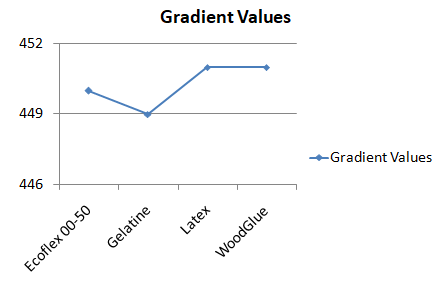
\includegraphics[scale=0.9]{Gradient.PNG}   
\caption{Graphical representation of gradient value obtained by each materials in the (ii) scenario}
\label{fig4.1}
\end{figure}

\begin{table}[h] 
\caption {Correct Rate and Error Rate obtained for CNN with feature vector as input} 
\label{tab:22} 
\center
\begin{tabular}{|c|c|c|}
\hline 
Materials Used (Live and Fake) & CR & ER\\ 
\hline 
Ecoflex 00-50 & 0.788 & 0.211 \\ 
\hline 
Gelatine & 0.808 & 0.192 \\ 
\hline 
Latex & 0.802 & 0.198 \\ 
\hline 
WoodGlue & 0.808 & 0.191 \\ 
\hline 
\end{tabular}
\end{table}

\chapter{Conclusion and Future Work}
The main limitation of many of the existing anti-spoof methods is the poor quality of the datasets obtained. The spoofing materials of poor image quality decreases the overall performance of the system. So we need either a best hardware for image acquisition or a good image processing method to obtain better results , but most of the hardware are expensive. 
\paragraph{}Here we proposed a method .....
The proposed WAT enhanced method yields an average accuracy of 85.8\%. The WAT enhanced image with minutiae features extracted, achieved an average accuracy of 79.8\%. We also computed the performance of CNN without any enhancement on image as input and obtained an average accuracy of 91.6\%.




% References Section
\renewcommand{\bibname}{REFERENCES}
\cleardoublepage % to clear the double page
\addcontentsline{toc}{chapter}{REFERENCES}	% to add reference to table of contents
\begin{spacing}{1.5}
\begin{thebibliography}{99}

\bibitem{1} \textbf{Tarang Chugh, Kai Cao, and Anil K. Jain}, ``Fingerprint Spoof Buster: Use of Minutiae-centered Patches,'' \textit{IEEE Transactions On Information Forensics And Security}, 2018.  

\bibitem{2} \textbf{Manisha Redhu and Dr. Balkisha}, ``Fingerprint Recognition Using Minutiae Extractor,'' \textit{International Journal of Engineering Research and Applications (IJERA)}, Vol. 3, Issue 4, Jul--Aug 2013.

\bibitem{3} \textbf{Emanuela Marasco and Arun Ross}, ``A Survey on Anti-spoofing Schemes for Fingerprint Recognition Systems,'' \textit{ACM Comput. Surv.}, 47, 2, Article 28, Nov 2014.

\bibitem{4} \textbf{Kumar Abhishek and Ashok Yogi}, ``A Minutiae Count Based Method for Fake Fingerprint Detection,'' \textit{Second International Symposium on Computer Vision and the Internet (VisionNet'15)}, 2015.

\bibitem{5} \textbf{Joshua J. Engelsma, Kai Cao, and Anil K. Jain}, ``RaspiReader: An Open Source Fingerprint Reader Facilitating Spoof Detection,'' \textit{Life Fellow, IEEE}, arXiv:1708.07887v1 [cs.CV], 25 Aug 2017.

\bibitem{6} \textbf{Athos Antonelli, Raffaele Cappelli, Dario Maio, and Davide Maltoni}, ``Fake Finger Detection by Skin Distortion Analysis,'' \textit{IEEE Transactions on Information Forensics and Security}, Vol. 1, No. 3, Sep 2006.

\bibitem{7} \textbf{Rodrigo Frassetto Nogueira, Roberto de Alencar Lotufo, and Rubens Campos Machado}, ``Fingerprint Liveness Detection using Convolutional Neural Networks,'' \textit{IEEE Transactions on Information Forensics and Security}, 1556-6013, 2015.

\bibitem{8} \textbf{Diego Gragnaniello, Giovanni Poggi, Carlo Sansone, and Luisa Verdoliva}, ``Fingerprint Liveness Detection based on Weber Local Image Descriptor,'' \textit{IEEE Journal}, 2013.

\bibitem{9} \textbf{Luca Ghiani, Gian Luca Marcialis, and Fabio Roli}, ``Fingerprint Liveness Detection by Local Phase Quantization,'' \textit{21st International Conference on Pattern Recognition (ICPR 2012)}, Nov 2012. 

\bibitem{10} \textbf{Samruddhi S. Kulkarni and Dr. Hemprasad Y. Patil}, ``A Fingerprint Spoofing Detection System Using LBP,'' \textit{International Conference on Electrical, Electronics, and Optimization Techniques (ICEEOT)}, 2016.

\end{thebibliography}
\end{spacing}
\bibliographystyle{unsrt}	
\nocite{*}


% Optional Appendix
\appendix
\chapter{Screen Shots}

\begin{figure}[htbp]
\centering
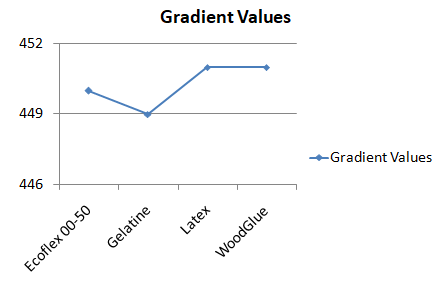
\includegraphics[scale=0.8]{Gradient.PNG}   
\caption{Sample visualization / Experimental gradient value}
\label{fig:sample_grad}
\end{figure}

% Note: Replace with your actual screenshot images when available
% \begin{figure}[htbp]
% \centering
% \includegraphics[width=0.8\textwidth]{liveimg.png}   
% \caption{Live fingerprint image from testing dataset}
% \label{fig:live_img}
% \end{figure}

\chapter{Sample Code}
\section*{Evaluation and Feature Extraction Script}

% Include code/text in verbatim environment to display exactly as written
\begin{verbatim}  
close all;
clear;
clc;

% 1. Read input image file
[filename, pathname] = uigetfile('*.png', 'Select an image', 'Dataset\Testing');
I = imread(fullfile(pathname, filename));
addpath('Waveatom');
val = wave(I);

% 2. Extract minutiae features
[rgbImage, ridge_xy, bifurcation_xy] = minutiaeextract(val);

% 3. Model prediction
if cnnPredict == 1
    uiwait(msgbox(sprintf('LIVE'), 'RESULT'));
else
    uiwait(msgbox(sprintf('FAKE'), 'RESULT'));
end
\end{verbatim}

\section*{Feature Extraction for Dataset Materials}
\begin{verbatim}
clc;
clear;

load fpsFs;
FList = ReadImageNames('DataSet');
Index = contains(FList, 'Testing\Fake\Ecoflex 00-50');
TestF_name_G = FList(Index, :);
TestF_G = fpsFs(Index, :);

net = trainSoftmaxLayer(TrainF', Ts);
[~, cnn_predict] = max(net(TestF'));
cp = classperf(TestL, cnn_predict);
\end{verbatim}


\end{document}